% Vilnius University beamer template
% Created in 2024 by Joana Katina

\documentclass[12pt]{beamer}
% You can use \documentclass[11pt,aspectratio=169]{beamer} 
% to adjust the aspect ratio to 16:9.
\renewcommand{\figurename}{}
\renewcommand{\tablename}{}
\renewcommand\thefigure{\arabic{figure} figure.}
\renewcommand\thetable{\arabic{table} table.}

\usepackage{graphicx}
\usepackage{listings}
\usepackage[
	backend=biber,
	style=numeric,
	sorting=ynt
]{biblatex}
\usepackage{algorithm,algorithmic}
\usepackage{caption}

\usepackage{biblatex}
\usepackage{hyperref}
\usepackage{subfig}

\addbibresource{references.bib}

\usetheme{Madrid}

\title[]{Title of the work}
\subtitle[]{Bachelor's thesis/Course work}
\author[Name Surname]{Name Surname}
\date{}

%% Supervisor
\addtobeamertemplate{author}{}{Supervisor: Pedagogical title Name Surname\par}

%% Scientific advisor - if not present or unknown, delete
\addtobeamertemplate{author}{}{Scientific advisor: Pedagogical title Name Surname\par}

%% Reviewer - if not present or unknown, delete
\addtobeamertemplate{author}{}{Reviewer: Pedagogical title Name Surname\par}

\setbeamertemplate{navigation symbols}{}
\titlegraphic{
\includegraphics[width=2cm]{resources/MIF.png}}

\usepackage{VUMIF}
\usepackage[T1]{fontenc}

%% Uncomment the section below to show a table of contents slide every time a new section starts
%% \AtBeginSection[]
%% {
%%  \begin{frame}<beamer>
%%  \frametitle{Table of contents}

%%% If you want the content to be shown only 1 time, delete the "    [currentsection]" part
%%  \tableofcontents[currentsection]

%%  \end{frame}
%% }


\begin{document}

\begin{frame}
    \titlepage
\end{frame}

\section{Examples of slides}

\begin{frame}{Example of an unnumbered list}
    \begin{itemize}
    \item Text text text text text text text text text text text text text text text text text text text text text text text text text text:
        \begin{itemize}
        \item Text text text text text text text text text text text text text text text text text text text text.
        \item Text text text text text text text text text text text text text text text text text text text text text text text text.
        \end{itemize}
    \item Text text text text text text text text text text text text text text text text text text text text text text text text text.
    \item Here, for example, is a quote for an article\cite{Januschowski_2020}.
    \item Here, for example, is a quote for a book\cite{Abraham_2009}.
    \end{itemize}
\end{frame}

\begin{frame}{Example of a numbered list}
    \begin{enumerate}
    \item Text text text text text text text text text text text text text text text text text text text text text text text text text text.
    \item Text text text text text text text text text text text text text text text text text text text text text text text text.
    \item Text text text text text text text text text text text text text text text text text text text text text text text text text.
    \item Text text text text text text text text text text text text text text text text text text text text text text text.
    \end{enumerate}
\end{frame}


\begin{frame}{Examples of formulas}
  Example formula:
  \begin{equation}
      \frac{\partial \overline{u_{i}} }{\partial t} + \overline{u_{j}} \frac{\partial \overline{u_{i}} }{\partial x_{j}} = -\frac{1}{\rho}\frac{\partial \overline{P}}{\partial x_{i}}+\nu\frac{\partial ^2\overline{u_{i}}}{\partial x_{j}\partial x_{j}}-\frac{\partial \overline{u_{i}'u_{j}'}}{\partial x_{j}}+\overline{g_{i}}
  \end{equation}
    Example formula:
  \begin{equation}
     \frac{\partial \overline{\phi}}{\partial t}+\overline{u_{i}}\frac{\partial \overline{\phi}}{\partial x_{i}}=\frac{\partial}{\partial x_{i}}(D\frac{\partial \overline{\phi}}{\partial x_{i}})-\frac{\partial (\overline{{u_{i}^{'}\phi^{'}}})}{\partial x_{i}}
  \end{equation}
\end{frame}

\begin{frame}{Example of table}
    Text text text text text text text text text text text text text text text text text text text text text text text text text text text text text text text text text text text text text text text text text text text text text text text text text text text text text text text text text text text text text text text text text text text text text text text text text text text text text text.
	\begin{table}
    	  \centering
        \caption{Example of table}
    	  \begin{tabular}{|c|c|c|}
    		\hline
    		\textbf{Header 1} & \textbf{Header 2} & \textbf{Header 3} \\
    		\hline
    		Cell 1-1 & Cell 1-2 & Cell 1-3 \\
    		\hline
    		Cell 2-1 & Cell 2-2 & Cell 2-3 \\
    		\hline
    		Cell 3-1 & Cell 3-2 & Cell 3-3 \\
    		\hline
    	  \end{tabular}
	\end{table}
\end{frame}

\begin{frame}{Example of image}
    \begin{center}
        \begin{columns}[onlytextwidth]
            \column{0.6\textwidth}
            \begin{itemize}
                \item The Pascaline consisted of balls on which the numbers 0 to 9 were written. The balls had prongs.
                \item After spinning once, the ball would hook onto the adjacent wheel and rotate it by one digit, i.e. the corresponding column of numbers would increase by one.
                \item B. Pascal's principle of "bound dials" has been used in almost every mechanical calculator developed over three centuries.
            \end{itemize}
            \column{0.4\textwidth}
            \begin{figure}
                \centering
                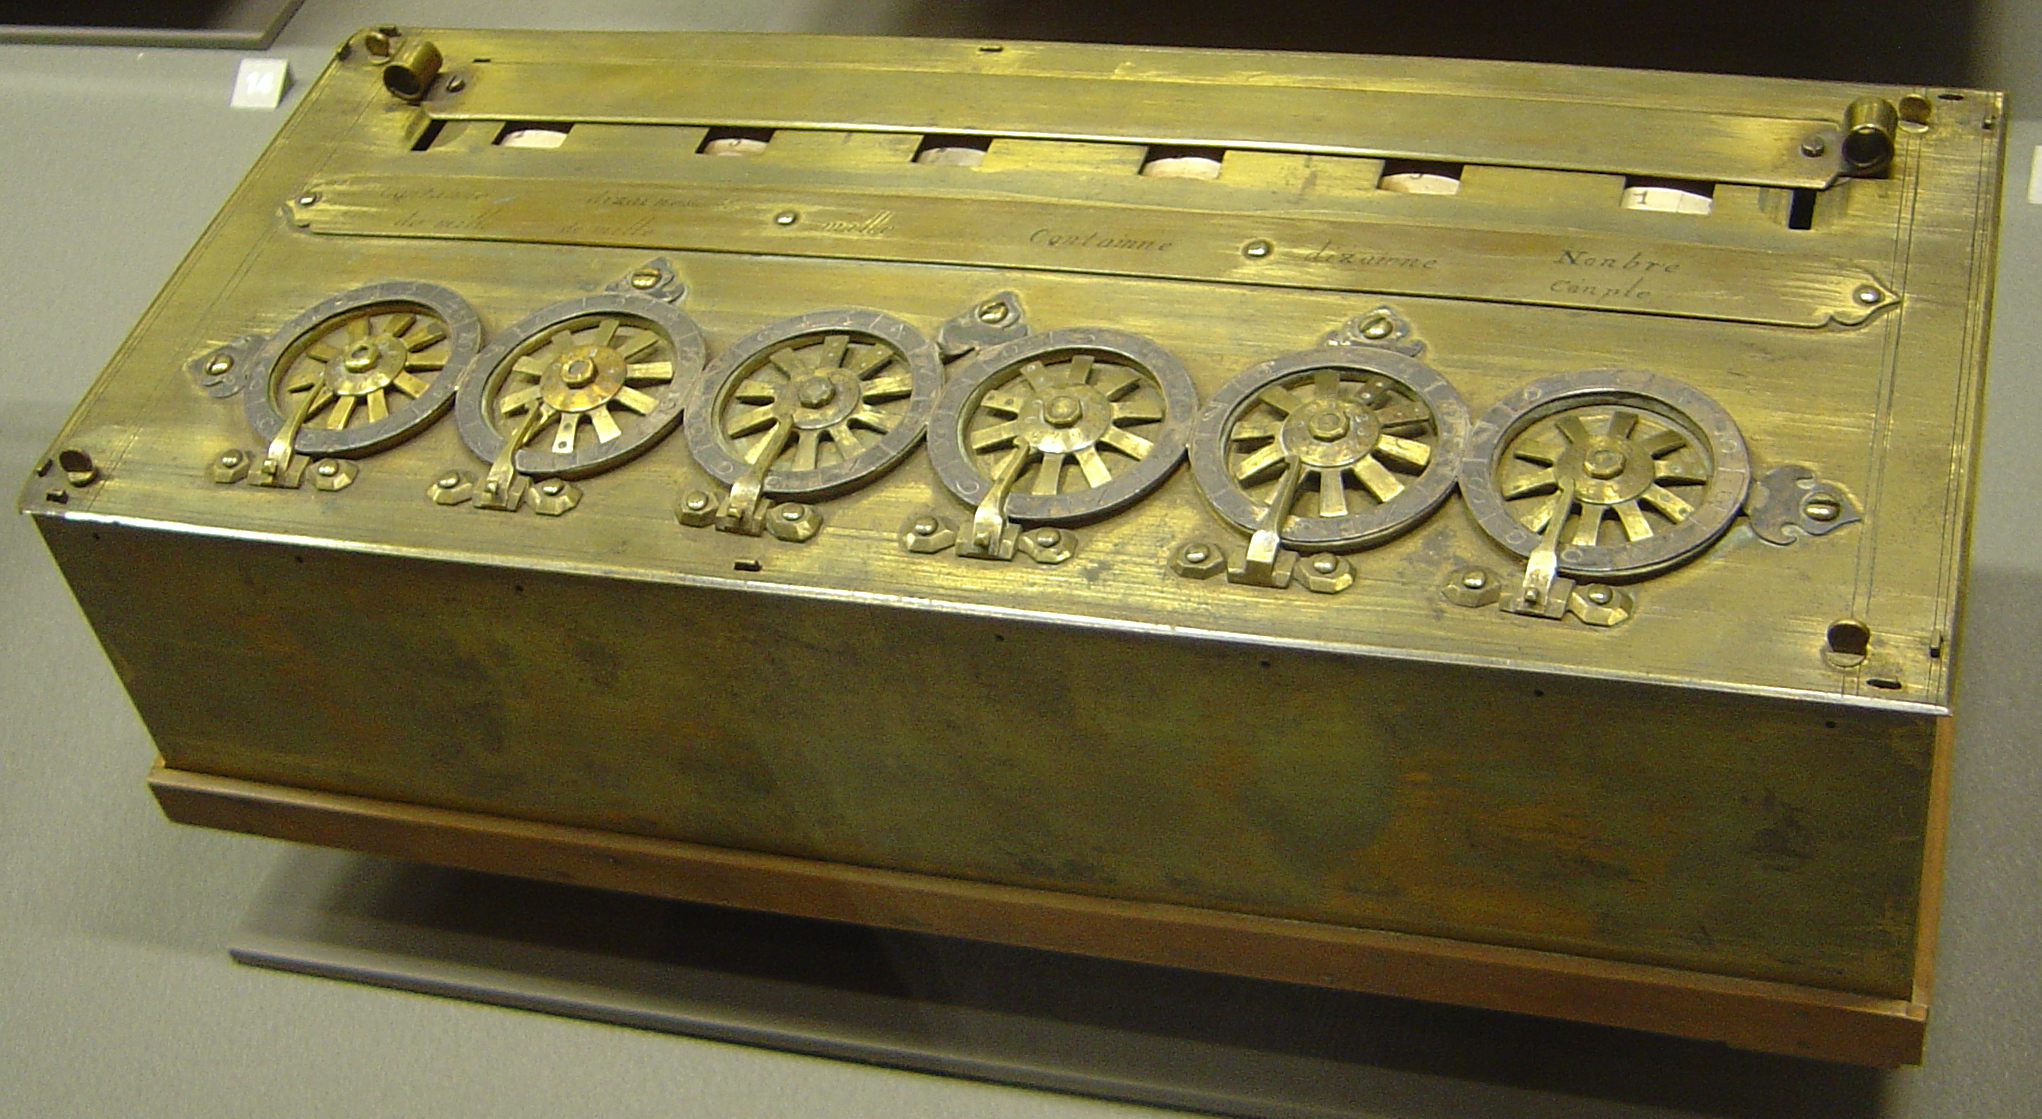
\includegraphics[width=0.9\textwidth]{resources/Pascaline.jpg}
                \caption[]{The Pascaline\cite{paskalina}}
            \end{figure}
        \end{columns}
    \end{center}
\end{frame}

\begin{frame}[allowframebreaks]{Two image example}
    The two pictures can be placed side by side.
    \begin{columns}[b]
        \column{0.5\textwidth}
        \begin{figure}
            \centering
            
\includegraphics[width=0.5\textwidth]{resources/MIF.png}
            \caption{VU MIF logo}
            \label{fig:mif-logo1}
        \end{figure}
        \column{0.5\textwidth}
        \begin{figure}
            \centering
            
\includegraphics[width=0.9\textwidth]{resources/VU_logo_lt.png}
            \caption{VU logo}
            \label{fig:vu-logo1}
        \end{figure}
    \end{columns}

\break

It is also possible to show two images side by side, making them share a common caption.

    \begin{figure}
        \subfloat[][VU MIF logo]{
        
\includegraphics[width=0.3\textwidth]{resources/MIF.png}
        \label{fig:mif-logo2}
    }
    \subfloat[][VU logo]{
        
\includegraphics[width=0.55\textwidth]{resources/VU_logo_lt.png}
        \label{fig:vu-logo2}
    }
    \caption{Common title for both images}
    \label{fig:two-images}
\end{figure}
\end{frame}

\begin{frame}{Example algorithm}
    Here is an example algorithm:
    \begin{algorithm}[H]
    \begin{algorithmic}[1]
    \FOR{$i=1$ to $N$}
    \FOR{$j=1$ to $JJJJ$}
    \STATE $energy[i*JJJ+j] =$ 
    $ interpolate(AAA[i*JJJ+j], ZZZ)$
    \ENDFOR
    \ENDFOR
    \end{algorithmic}
    \caption{pseudocode for the calculation of}
    \label{alg:seq}
    \end{algorithm}
\end{frame}

\section{Literature sources}
\begin{frame}[t,allowframebreaks]
    \frametitle{Literature sources}
    \printbibliography
\end{frame}

\end{document}
